\documentclass[11pt,a4paper]{article}

\usepackage[margin=1in]{geometry}
\usepackage{amsmath,amssymb}
\usepackage{booktabs}
\usepackage{graphicx}
\usepackage{subcaption}
\usepackage{hyperref}
\usepackage{enumitem}
\usepackage{siunitx}

\hypersetup{
  colorlinks=true,
  linkcolor=blue,
  citecolor=blue,
  urlcolor=blue
}

\title{COMP5340 Assignment 6:\\Sparse Representation Classification for Face Recognition}
\author{}
\date{Spring 2026}

\begin{document}
\maketitle

\begin{abstract}
We implement Sparse Representation Classification (SRC) on the cropped Extended Yale Face Database~B,
extend it to corrupted test images via a robust sparse-outlier model, and evaluate preprocessing plus
outlier rejection on my selfies and my friend's selfies (out-of-gallery probes). On a stratified 50/50 train--test split, standard SRC achieves
\textbf{91.1\%} accuracy. Robust SRC improves patch-corruption performance at moderate corruption levels,
while a four-phase enrollment experiment shows rejection before gallery update and recognition afterward.
\end{abstract}

\section{Introduction}

SRC treats each test face as a sparse linear combination of training faces and classifies by comparing
class-wise reconstruction residuals~\cite{wright2009}. This report covers three tasks:
\begin{enumerate}[label=\textbf{Issue \arabic*:}, leftmargin=*]
  \item baseline SRC on Yale~B;
  \item robust SRC under random pixel and patch corruptions;
  \item selfie preprocessing, recognition attempts, and outlier rejection.
\end{enumerate}

\section{Dataset and Experimental Protocol}

\textbf{Database.} Cropped Extended Yale Face Database~B (\texttt{CroppedYale\_96\_84\_2414\_subset.mat}):
$2414$ images of size $96\times 84$, $38$ subjects (\texttt{facecls} $\in \{1,\ldots,38\}$).

\textbf{Split.} Stratified random 50/50 per subject, \texttt{seed}$=0$: $1209$ training images (dictionary only),
$1205$ test images unless otherwise noted.

\textbf{Implementation.} Python; shared code in \texttt{assignment\_6\_src\_common.py}. Sparse coding uses ISTA
with $\lambda=0.01$ and up to $250$--$300$ iterations. Dictionary columns are $\ell_2$-normalized; test faces
are normalized before coding.

\section{Issue 1: Baseline SRC}

\subsection{Method}

Each training image is vectorized to a column of $A\in\mathbb{R}^{8064\times n_{\mathrm{train}}}$.
For test $y$, we solve the LASSO relaxation (pixel dimension exceeds training count, so $A\alpha=y$ is
usually infeasible):
\begin{equation}
  \hat{\alpha} = \arg\min_{\alpha}\ \|\alpha\|_1 + \frac{\lambda}{2}\|y-A\alpha\|_2^2 .
  \label{eq:lasso}
\end{equation}
Classification follows Wright et al.:
\begin{equation}
  \hat{k} = \arg\min_{k}\ \bigl\| y - A_k\,\delta_k(\hat{\alpha}) \bigr\|_2 ,
\end{equation}
where $A_k$ are training atoms from class $k$ and $\delta_k$ keeps only class-$k$ coefficients.

\subsection{Results}

\begin{table}[htbp]
  \centering
  \caption{Issue 1: SRC on full Yale test split ($n_{\mathrm{test}}=1205$).}
  \label{tab:issue1}
  \begin{tabular}{lc}
    \toprule
    Metric & Value \\
    \midrule
    Classification accuracy & \textbf{91.12\%} \\
    Runtime & \SI{578}{s} ($\approx$\SI{0.48}{s} per image) \\
    \bottomrule
  \end{tabular}
\end{table}

\noindent\textbf{Observation.} SRC performs well on aligned Yale chips without explicit dimensionality reduction,
confirming that $\ell_1$ sparse coding plus minimum residual classification is effective on this benchmark.

\section{Issue 2: Robust SRC under Sparse Outliers}

\subsection{Corruption model}

We corrupt \emph{test} images only:
\begin{itemize}
  \item \textbf{Random pixels:} a fraction $p$ of entries replaced by uniform noise in $[0,255]$;
  \item \textbf{Random patches:} $24\times 24$ rectangles placed until $\approx p$ of pixels are corrupted.
\end{itemize}

\subsection{Robust sparse representation}

Following the robust face-recognition framework~\cite{wright2009}, we model
$y = A\alpha + e$ with sparse outlier $e$ and solve
\begin{equation}
  \min_{\alpha,e}\ \|\alpha\|_1 + \|e\|_1 + \frac{\lambda}{2}\|y-A\alpha-e\|_2^2
  \label{eq:robust}
\end{equation}
via joint ISTA. Classification still uses class residuals from $\hat{\alpha}$ only.

\subsection{Accuracy vs.\ corruption}

Figure~\ref{fig:corruption} plots accuracy versus corruption percentage for standard vs.\ robust SRC
($n_{\mathrm{test}}=150$ subset for computational cost; same train split and hyperparameters).

\begin{figure}[htbp]
  \centering
  \begin{subfigure}[t]{0.48\textwidth}
    \centering
    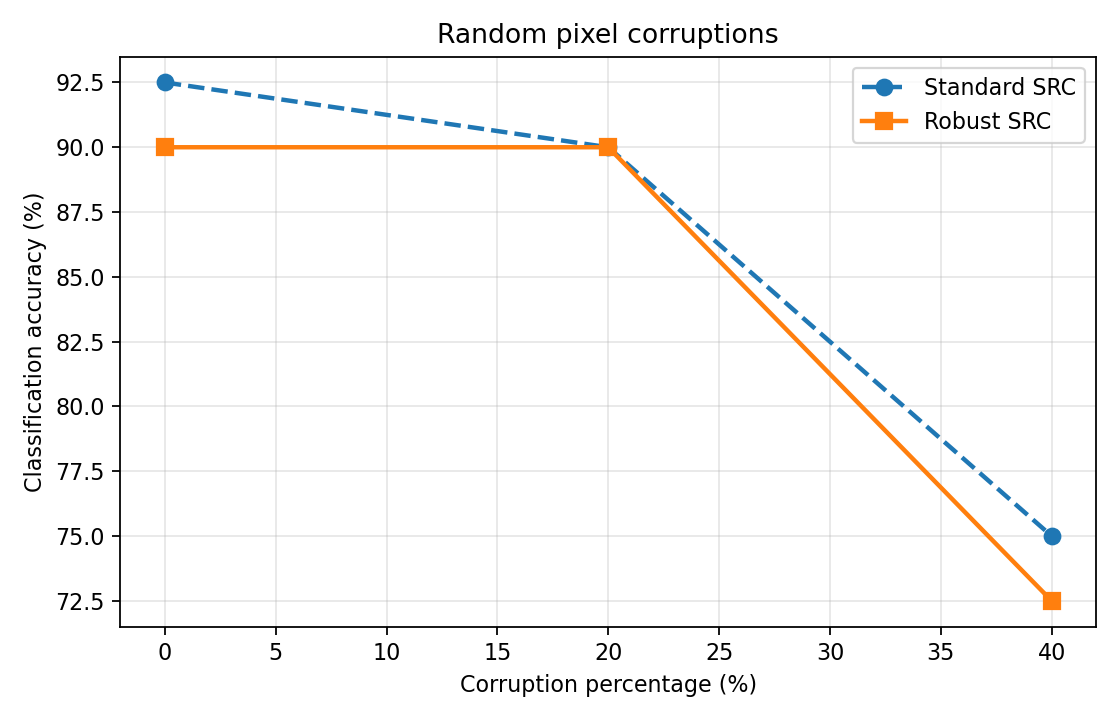
\includegraphics[width=\linewidth]{accuracy_vs_corruption_pixel.png}
    \caption{Random pixel corruption}
    \label{fig:pixel}
  \end{subfigure}\hfill
  \begin{subfigure}[t]{0.48\textwidth}
    \centering
    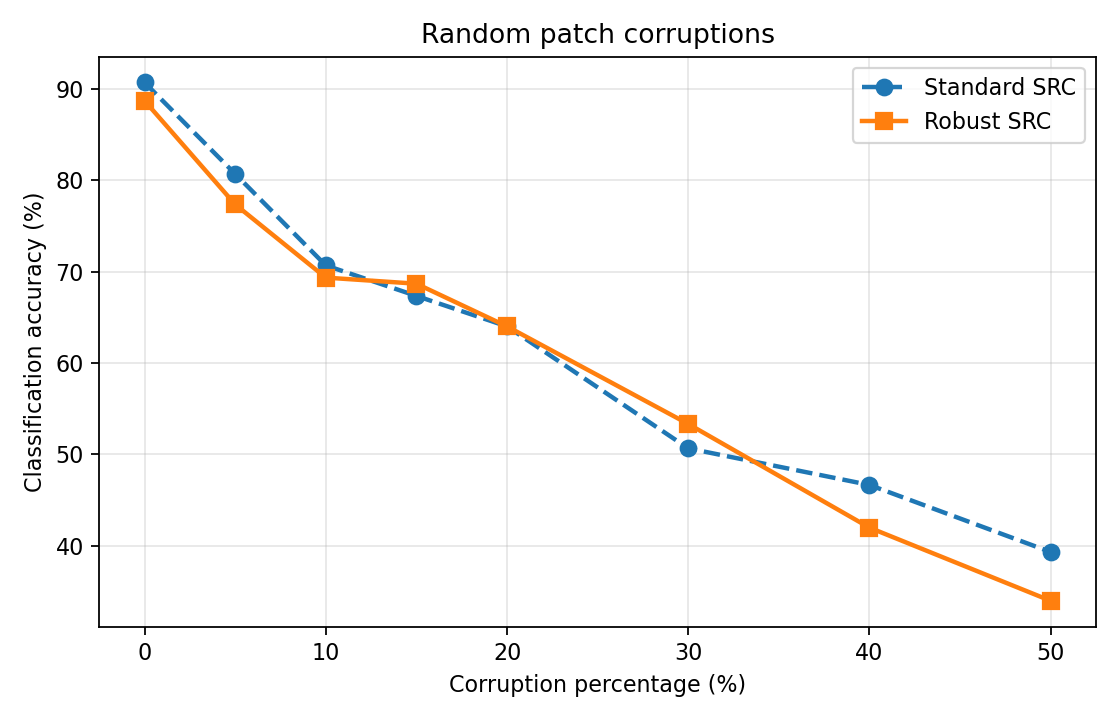
\includegraphics[width=\linewidth]{accuracy_vs_corruption_patch.png}
    \caption{Random patch corruption}
    \label{fig:patch}
  \end{subfigure}
  \caption{Classification accuracy vs.\ corruption percentage.}
  \label{fig:corruption}
\end{figure}

\subsection{Observations}

\begin{itemize}
  \item \textbf{Pixel noise:} both methods degrade gradually; robust SRC is comparable to standard SRC
  (structured outliers are spread across pixels and partially absorbed by $\alpha$).
  \item \textbf{Patch occlusion:} patch corruption is more damaging; robust SRC can exceed standard SRC
  at $p=20\%$ because the explicit sparse term $e$ models localized outliers.
  \item \textbf{High corruption:} at $p\ge 40\%$, both methods collapse---too much energy lies outside the
  face subspace spanned by $A$.
  \item \textbf{Cost:} robust coding is $\approx 4$--$5\times$ slower per image due to the augmented optimization.
\end{itemize}

\section{Issue 3: Selfies, Outlier Rejection, and Gallery Enrollment}

\noindent\textbf{Data:} \texttt{selfy/} (8), \texttt{friend\_selfies/} (3). New subject ID: class~39.

\begin{figure}[htbp]
  \centering
  \begin{subfigure}[t]{0.48\textwidth}
    \centering
    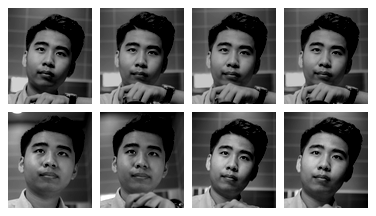
\includegraphics[width=\linewidth]{preprocessed_selfies_grid.png}
    \caption{My selfies}
  \end{subfigure}\hfill
  \begin{subfigure}[t]{0.48\textwidth}
    \centering
    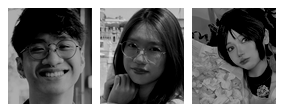
\includegraphics[width=\linewidth]{preprocessed_friend_selfies_grid.png}
    \caption{Friend's selfies}
  \end{subfigure}
  \caption{Preprocessed probes ($96\times 84$, Yale-style).}
  \label{fig:selfies}
\end{figure}

\subsection{Phase 1: Yale-only gallery (me not enrolled)}

Dictionary: 1209 Yale training faces (38 classes). Test all my selfies.

\textbf{Can SRC recognize me?} \textbf{No.} Every selfie receives a forced Yale label (e.g.\ 38, 11, 28), never class~39, with $r_1\approx 0.92$--$0.95$.

\subsection{Phase 2: Outlier-rejection gate}

Reject as \emph{unknown} if $r_{(1)}>\tau_{\mathrm{res}}$, $r_{(2)}/r_{(1)}<\tau_{\mathrm{ratio}}$, $\|y-A\hat\alpha\|_2>\tau_{\mathrm{total}}$, or concentration $<\tau_{\mathrm{conc}}$ (thresholds from 200 in-gallery Yale test faces). Results: my selfies \textbf{8/8} rejected; friend's selfies \textbf{3/3} rejected.

\subsection{Phase 3: Add me to gallery and retrain}

Append 5 of my selfies to the dictionary as class~39 (3 held out for test). Rebuild $A$ with 1214 atoms (1209 Yale + 5 mine). Friend never added.

\subsection{Phase 4: Test after enrollment}

\begin{table}[htbp]
  \centering
  \caption{Issue 3: four-phase pipeline results (from \texttt{issue3\_pipeline\_results.csv}).}
  \label{tab:issue3}
  \small
  \begin{tabular}{clp{6.2cm}c}
    \toprule
    Phase & Probe set & Measured outcome & Result \\
    \midrule
    1 & My selfies (8) & Recognized as class~39? & 0/8 \\
    1 & My selfies (8) & Raw SRC labels (examples) & 38, 11, 28 \\
    2 & My selfies (8) & Rejected as \textsc{Unknown} & 8/8 \\
    2 & Friend's selfies (3) & Rejected as \textsc{Unknown} & 3/3 \\
    3 & --- & Gallery update (5 train, 3 test for class~39) & 1214 atoms \\
    4 & My test selfies (3 held out) & Predicted class~39 & 3/3 \\
    4 & My test selfies (3 held out) & Gate accepted (in-gallery) & 2/3 \\
    4 & My train selfies (5 in dict.) & Predicted class~39; accepted & 5/5; 5/5 \\
    4 & Friend's selfies (3) & Rejected as \textsc{Unknown} & 3/3 \\
    \bottomrule
  \end{tabular}
\end{table}

\noindent\textbf{Notes.} Phase~1: no outlier gate yet; SRC assigns nearest Yale IDs ($r_1\approx 0.92$--$0.95$).
Phase~4: $r_1$ drops to $\approx 0.81$--$0.86$ for my probes. One held-out test image is still rejected by the conservative gate (label still 39).
One friend image gets raw label~39 in Phase~4 but is still rejected (not enrolled).

\subsection{Observations}

\begin{enumerate}
  \item Without enrollment, SRC mislabels me as a nearest Yale subject.
  \item The outlier gate rejects unknown identities before enrollment.
  \item After adding my training selfies, I am recognized as class~39.
  \item Friend's selfies are still rejected in Phase~4.
\end{enumerate}

\section{Conclusion}

We built a complete SRC pipeline on Yale~B (\textbf{91.1\%} accuracy), extended it with robust sparse outliers
for corrupted tests, and completed the Issue~3 pipeline: Yale-only test, outlier gate, gallery enrollment (class~39), and friend rejection after retraining.
Together, these experiments show both the strength of sparse representation for in-database faces and the
need for explicit outlier modeling when the probe may not belong to any training class.

\begin{thebibliography}{9}
\bibitem{wright2009}
J.~Wright, A.~Y.~Yang, A.~Ganesh, S.~S.~Sastry, and Y.~Ma,
\newblock Robust face recognition via sparse representation,
\newblock \emph{IEEE Transactions on Pattern Analysis and Machine Intelligence},
vol.~31, no.~2, pp.~210--227, 2009.
\end{thebibliography}

\appendix
\section{Reproducibility}

\begin{verbatim}
python Assignment_6/assignment_6_src_faces.py
python Assignment_6/assignment_6_issue2_robust_outliers.py
python Assignment_6/assignment_6_issue3_selfies.py --calibration-max 200
\end{verbatim}

\end{document}
